\documentclass[../../relatorio.tex]{subfiles}

\begin{document}

\subsection{Reservas Internacionais em USD}

\begin{figure}[ht]
  \begin{minipage}{0.30\textheight}
    \centering
      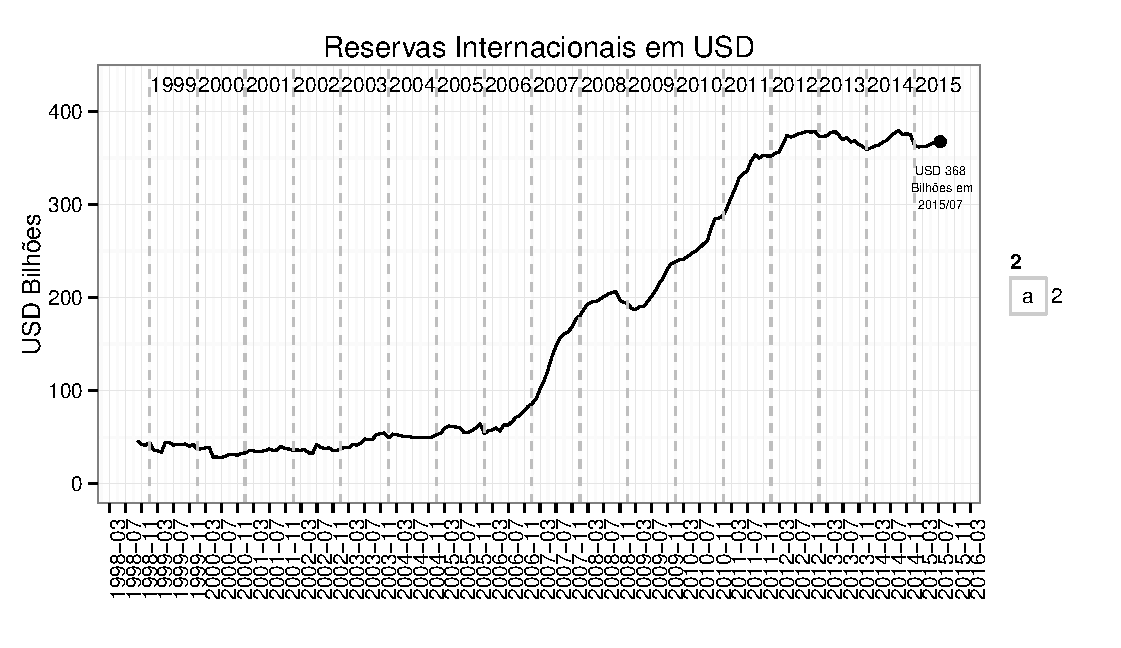
\includegraphics{ReservasUSD.pdf}
  \end{minipage}
\end{figure}

As reservas internacionais são os depósitos em moeda estrangeira dos bancos centrais e autoridades monetárias. São ativos dos bancos centrais que são mantidos em diferentes reservas, como o dólar americano, o euro ou o iene, e que são utilizados no cumprimento dos seus compromissos financeiros, como a emissão de moeda, e para garantir as diversas reservas bancárias mantidas num banco central por governos ou instituições financeiras. \footnote{http://pt.wikipedia.org/wiki/Reservas\_internacionais}


\pagebreak

\end{document}
